
\question 
%
%The denominator of the propagators of many gauge-bosons takes the  $$q^2-m^2.$$
%
In the simplified Feynman rules given in the lecture course, the propagators  for the photon and $W$-boson were given as
$$
-\frac {i g_{\mu\nu}}{q^2}
\ \ \text{and} \ \ 
-\frac{i\left(g_{\mu\nu}-q^\mu q^\nu/m_W^2\right)}{q^2-m_W^2}
$$
respectively.  Both have a denominator of the form $q^2-m^2$.
\begin{allparts}
\part
Comment on the circumstances in which it might be reasonable to replace  $q^2-m^2$ in the denominator of a propagator with $q^2-m^2+i m\Gamma$, explaining what $\Gamma$ might mean in this context.\marks{4}
\answer

I expect here some comments relating to page 497 of the lecture handout where the Breit-Wigner resonance was discussed in connection with the modelling of an unstable particle which decay rate $\Gamma$ (which ends up also turning out to be its width). There the replacement of $m$ with $m-i\Gamma/2$ was shown to effect the appropriate decay in probability of existence as a function of time, and was shown to changing $q^2-m^2$ to $q^2-m^2+i m\Gamma + \frac 1 4 \Gamma^2$ which resembles  $q^2-m^2+i m\Gamma$ if $\Gamma\ll m$.  A student might also mention that in principle no such insertion might be needed in Feynman-rule propagators since the inclusion of all diagrams at all orders should lead to the removal of the denominator=0  singularity .... however the $q^2-m^2\rightarrow q^2-m^2+i m\Gamma$ goes a long way to giving us a pragmatic way of calculating some reasonable results at first order, and so these insertions are often made.
\endanswer
\end{allparts}
Now suppose that there exist Bogus universes containing only electrons, positrons, muons, antimuons and Bogons, and that interactions are described by a theory called Quantum Bogodynamics (or QBD for short). Suppose that QBD is identical to QED except that: (i) photons are replaced by Bogons, (ii) there are two types of Bogon instead of one type of photon, and (iii) in some universes Bogons can be massive  ($0\le m_1\le m_2$).  Furthermore, suppose that the coupling strengths $e_1$ and $e_2$ for the two types of Bogon need neither be equal nor have the same sign.  In short, you may assume that in any Bogus universe the QBD Feynman rules have propagator and vertex factors for the $k^\text{th}$ type of Bogon as follows:
\alig{
\vcenter{\hbox{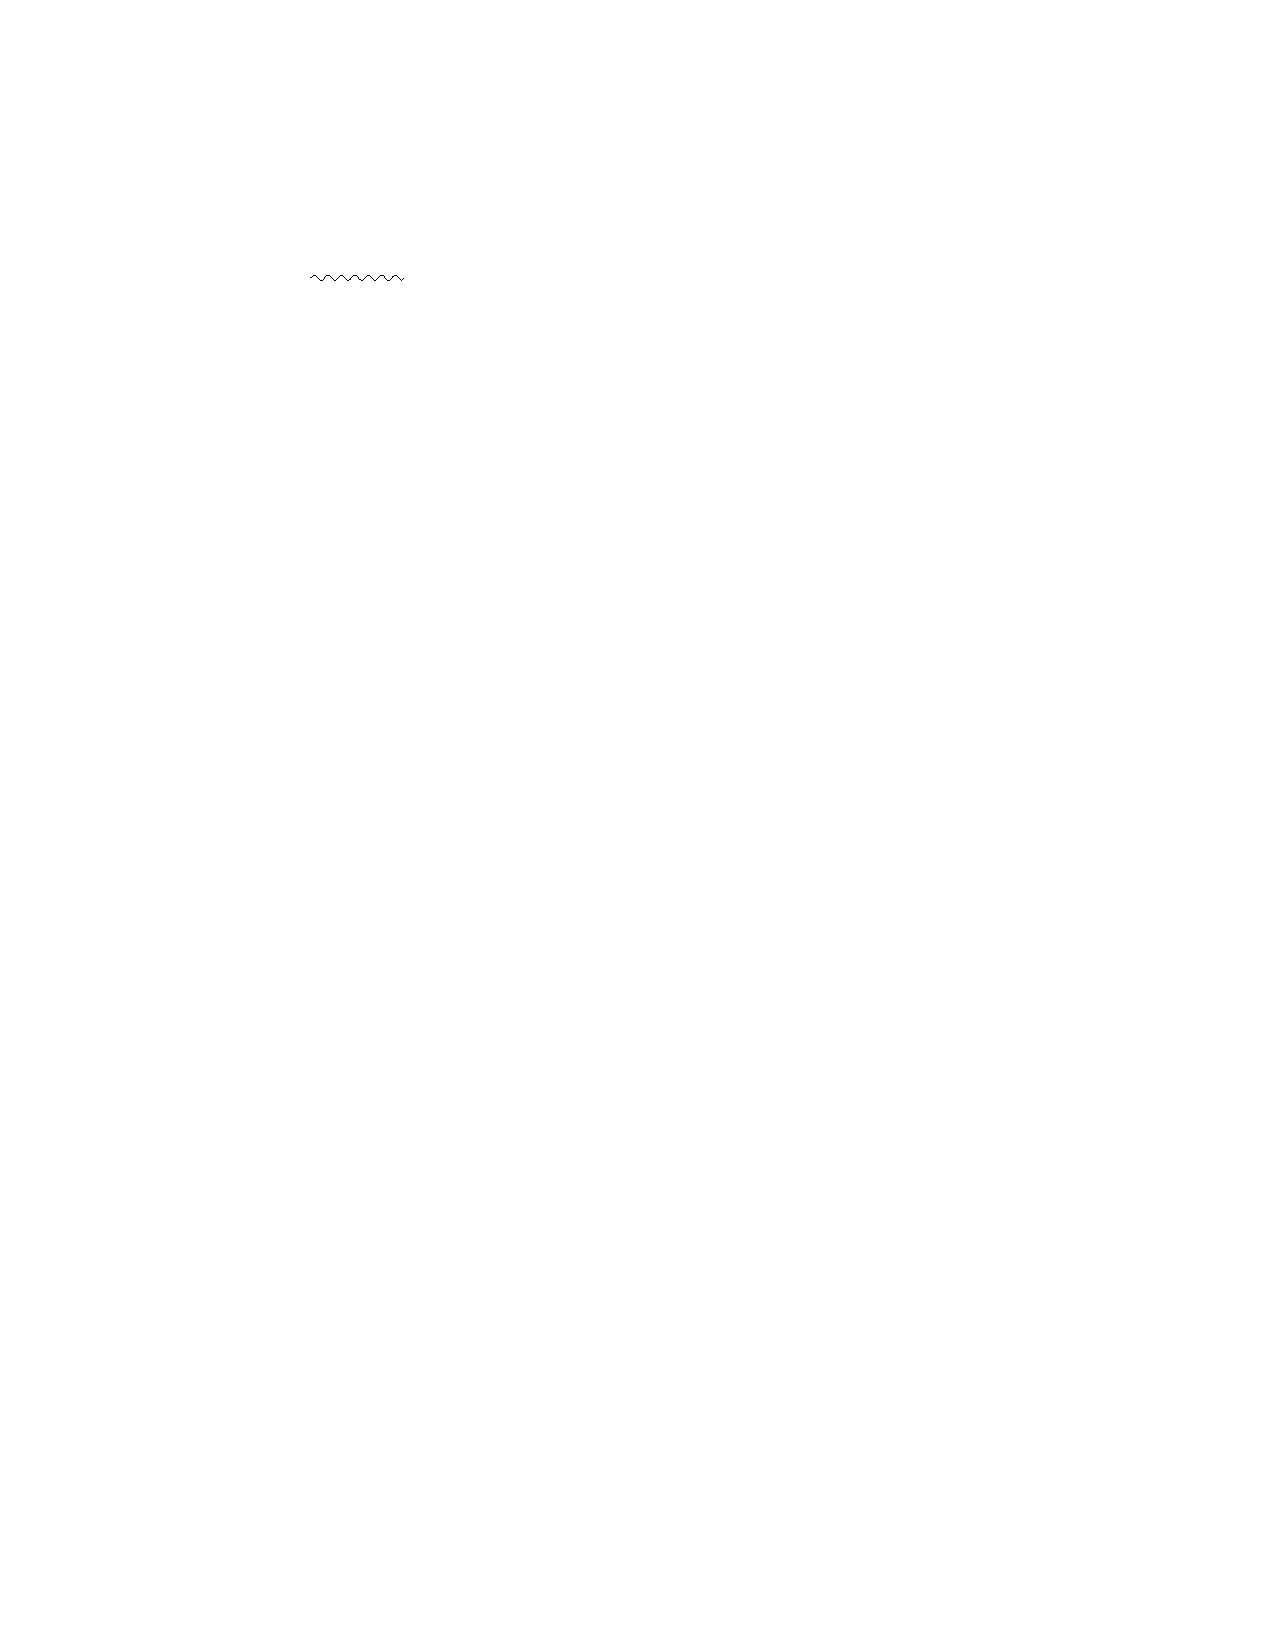
\includegraphics{Diagrams/photon.pdf}}}={
\frac{-i g_{\mu\nu}}{q^2-m_k^2+i m_k \Gamma}
},
%\right]
\qquad\text{}\qquad 
%\left[
\vcenter{\hbox{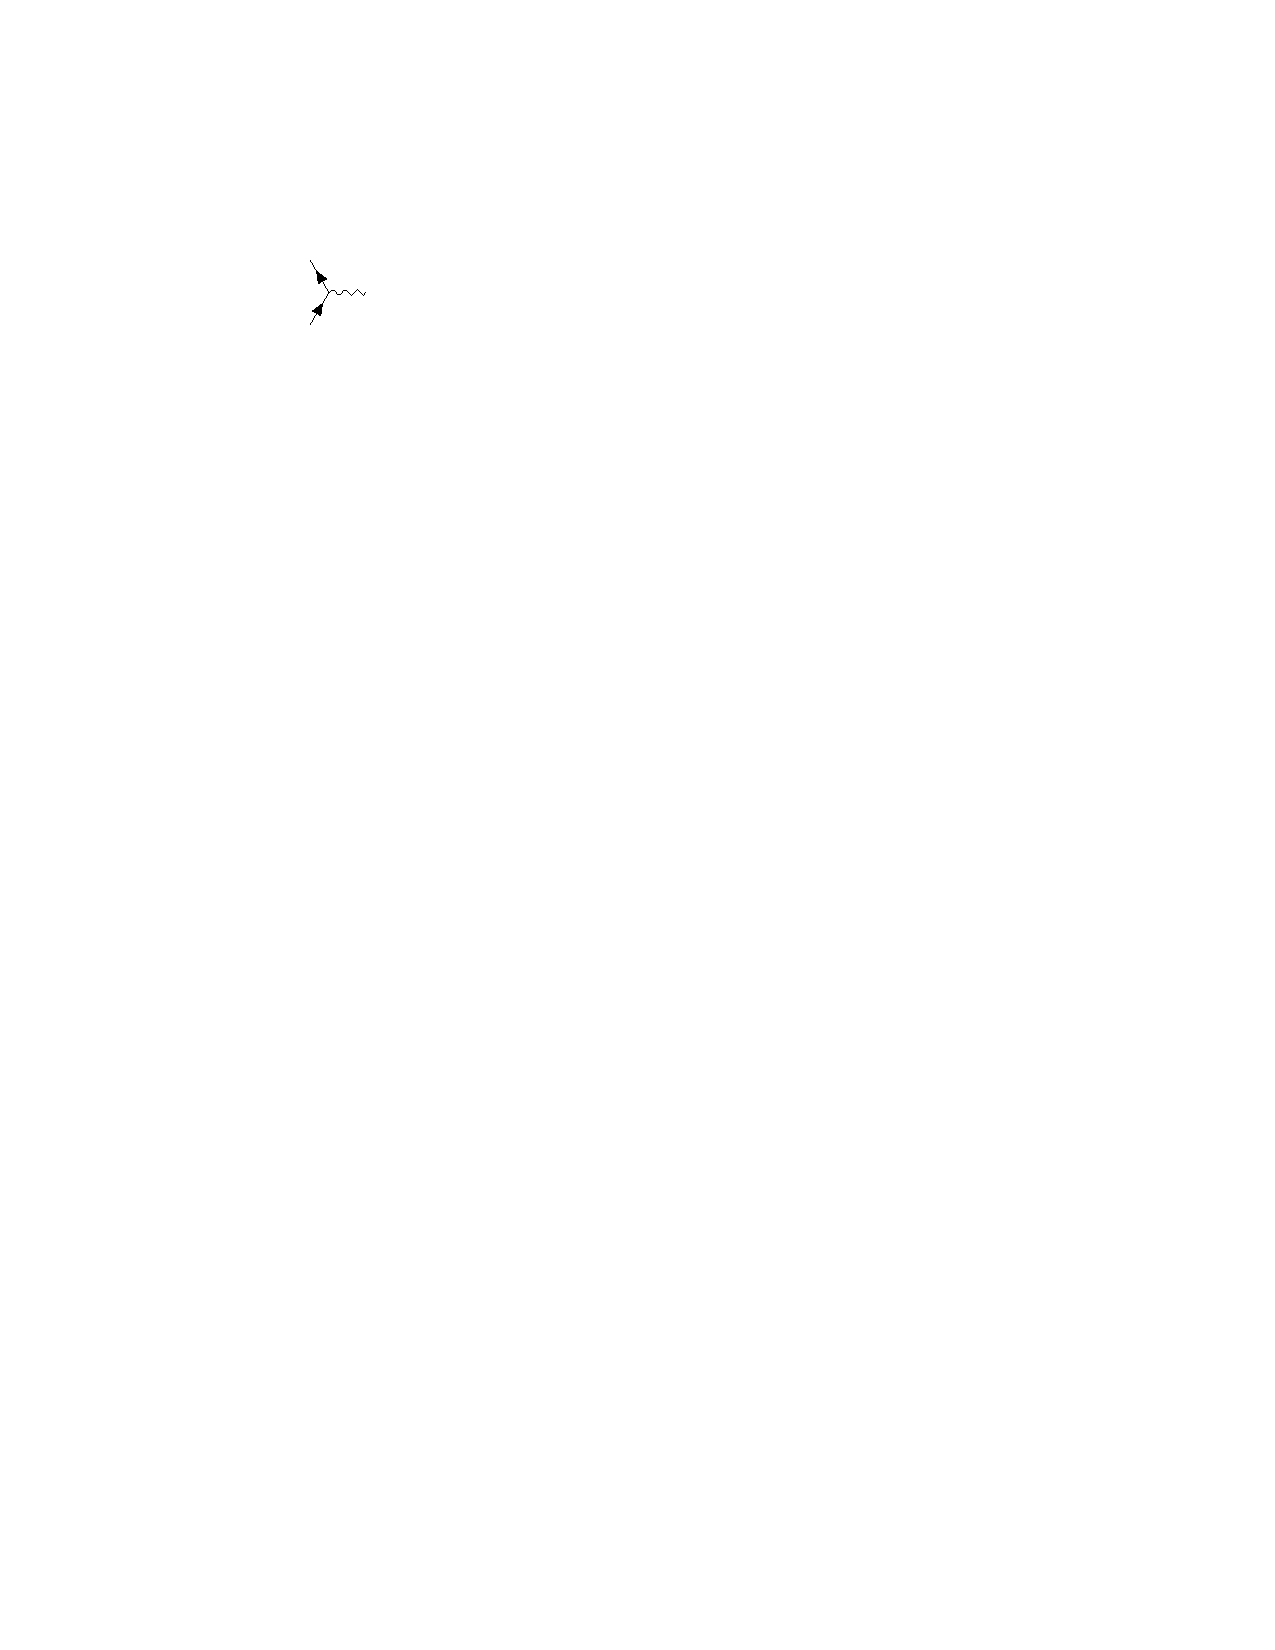
\includegraphics{Diagrams/eeg_vertex.pdf}}}={
i e_k \gamma^\mu
}
%\right]
%\qquad\text{respectively.}
\nonumber
}
where $\Gamma\ge0$ is a non-negative constant.
\begin{allparts}
\part
In a universe in which $0<m_1=m_2$, $0<\Gamma\ll m_1$ and $e_1 e_2>0$,  would it be possible for Bogus physicists looking at $e^+e^-\rightarrow \mu^+\mu^-$ data to determine that there are two types of Bogon rather than one?
Would anything change if we were to consider instead $e_1 e_2<0$ ? \marks{4}
\answer

The main point to make would be that any matrix element featuring one Bogon could be added to another having the other sort of Bogon substituted for it. Therefore every matrix element having an $\frac{e_1^2}{q^2-m^2+im\Gamma}$ (with the $e_1$ being squared as there will be a vertex factor at each end of the same Bogon) will end up added to another such that the resulting total matrix element would contain only terms of the form $\frac{e_1^2+e_2^2}{q^2-m^2+im\Gamma}$. Such a matrix element would be phenomenologically  indistinguishable from one derived from a theory in which there was only one bogon having single larger coupling constant $e$ satisfying $e^2=e_1^2+e_2^2$. Therefore there would be no way of deducing the existence of one rather than two Bogons.  Note that because of the presence of the squares of the coupling constants, signs are a red-herring here.
\endanswer
\end{allparts}
Suppose there are two Bogus universes $A$ and $B$, and that in each of these universes $0< m_1 < m_2$, $\Gamma=0$ and $e_1$ is equal to a non-zero constant $e$.  Further suppose that Universe $A$ has $e_2=0$ while Universe $B$ has $e_2=e$.  
\begin{allparts}
\part
For which range(s) of $\sqrt s$ (if any) is the tree-level cross section for the process $e^+ e^- \rightarrow \mu^+ \mu^-$ bigger in Universe $A$ than in Universe $B$, and for which range(s) of $\sqrt s$ (if any) is the reverse true?\marks{16}
\answer



The matrix element for $e^+e^-\rightarrow \mu^+\mu^-$ via two interfering massive bosons will be proportional to \alig{
j_e j_\mu \left(
\frac {e_1^2} {q^2-m_1^2+i m_1 \Gamma}
+
\frac {e_2^2} {q^2-m_2^2+i m_2 \Gamma}
\right)
}which is proportional to
\alig{e_1^2 z_1+e_2^2 z_2}where
\alig{
z_1&=
\frac 1 {q^2-m_1^2+i m_1 \Gamma}
%=
%\frac {q^2-m_1^2-i m_1 \Gamma } {(q^2-m_1^2)^2+ m_1^2 \Gamma^2}
%=
%\frac {q^2-M^2-i \epsilon M^2  } {(q^2-M^2)^2+ \epsilon^2M^4 %}
,\qquad\text{and}\\
z_2&=
\frac 1 {q^2-m_2^2+i m_2 \Gamma}
%=
%\frac {q^2-m_2^2-i m_2 \Gamma } {(q^2-m_2^2)^2+ m_2^2 \Gamma^2}
%=
%\frac {q^2-(2M)^2-i 2\epsilon M^2  } {(q^2-(2M)^2)^2+ 4\epsilon^2 M^4 }.
}
%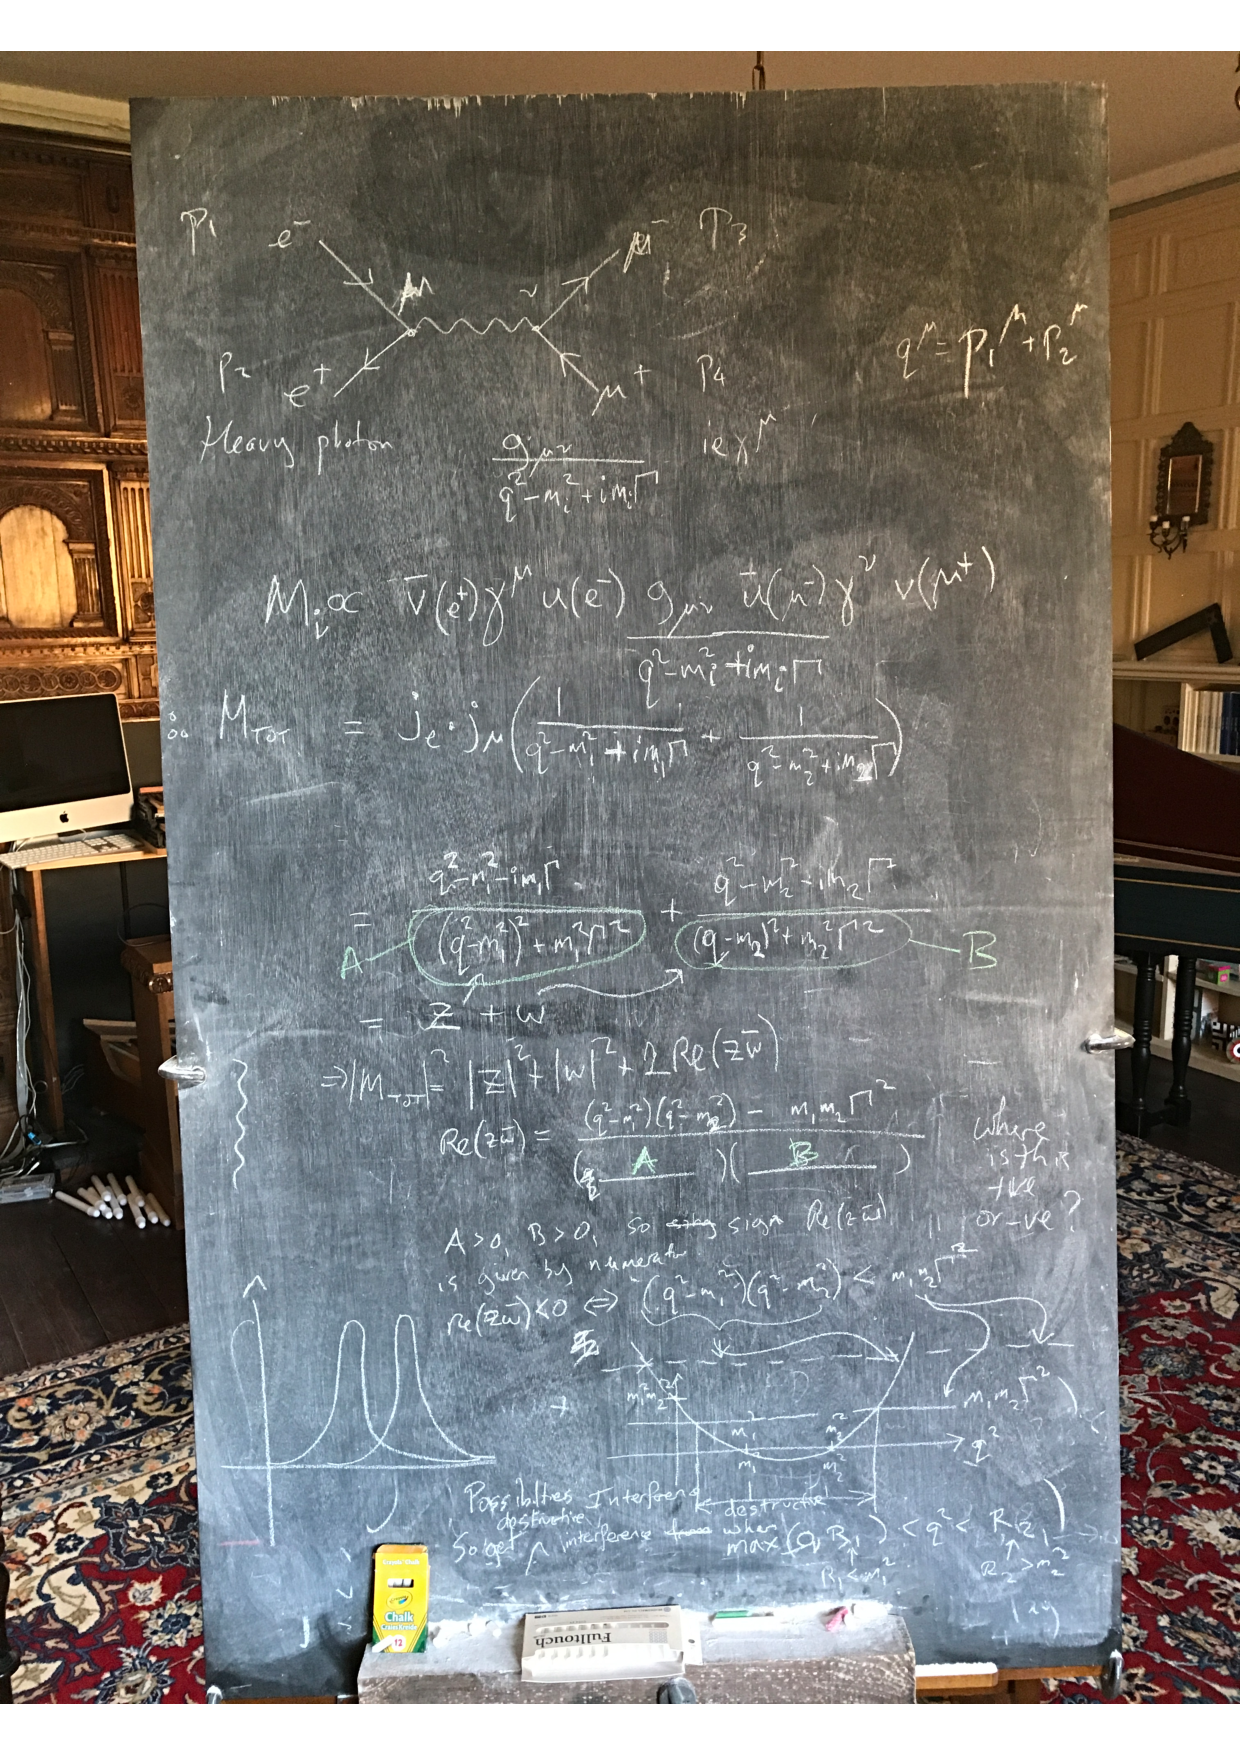
\includegraphics[height=15cm,width=15cm]{BogonMathsSketch}
%in either universe\alig{
%|M_{\text{tot}}|^2 
%&\propto
%|z_1+z_2|^2
%\\
%&=
%|z_1|^2
%+|z_2|^2
%+2 \Re\left[{z_1 z_2^*}\right]
%}and therefore
and hence\alig{
|M_{\text{tot}}|^2
&\propto |j_e\cdot j_\mu|^2\left|
e_1^2 z_1 + e_2^2 z_2
\right|^2
\\
&\propto\left|
e_1^2 z_1 + e_2^2 z_2
\right|^2.
}
If we consider the case which is mentioned in the question with  $\Gamma=0$, the complex numbers disappear from the question and we are left with
\alig{
|M_{\text{tot}}|^2
&\propto
\left(
e_1^2 z_1 + e_2^2 z_2
\right)^2
}
and hence, comparing the cross sections in the two universes\footnote{It is important to note that in this particular calculation only \textit{positive} constants has been dropped at each use of a proportional symbol ($\propto$).}:\alig{
\sigma_B-\sigma_A
&\propto
|M_{\text{tot(B)}}|^2
- 
|M_{\text{tot(A)}}|^2\nonumber
\\
&\propto
\left(
e^2 z_1 + e^2 z_2
\right)^2
-
\left(
e^2 z_1 + 0^2 z_2
\right)^2\nonumber
\\
&=
e^4\left(  (z_1+z_2)^2 - z_1^2\right)\nonumber
\\
&\propto
z_2^2+2 z_1 z_2\nonumber
\\
&=
z_2^2\left(1+\frac {2 z_1} {z_2}\right)\nonumber
\\
&=
1+\frac {2 z_1} {z_2}\label{eq:thingsketched}
}and hence\alig{
\left(\sigma_B >\sigma_A\right)
&\iff
\left( 1+\frac {2 z_1} {z_2} > 0\right)
\\
&\iff
\left(
1+\frac {2 (s-m_2^2)} {s-m_1^2} 
> 0\right).\label{eq:cond45}
}
The condition in \eqref{eq:cond45} is trivially true if both terms on the denominator have the same sign, which (given that $m_1^2<m_2^2$) happens if $\sqrt s<m_1$ or $\sqrt s>m_2$.  The only uncertainty relates to what happens when $s$ is in the intermediate position: $m_1^2 \le s \le m_2^2$. In this intermediate zone we have:
\alig{
\left(
1+\frac {2 (s-m_2^2)} {s-m_1^2} 
> 0\right)
&\iff
\left(
(s-m_1^2)+2 (s-m_2^2)  
> 0\right)
\\
&\iff
\left(
3s  
> m_1^2+2m_2^2
\right)
\\
&\iff
\left(
\sqrt s  > \sqrt{\frac 1 3 \left(m_1^2+2m_2^2\right)
}\right)
}therefore, considering all non-negative $\sqrt s$ we see that
\alig{
\left(\sigma_B \le \sigma_A\right)
&\iff
\left[
m_1\le\sqrt s\le\sqrt{\frac 1 3 \left(m_1^2+2m_2^2\right)}
\right]
}which is perhaps best summarized in the following sketches (in which the quantity on the RHS of  \eqref{eq:thingsketched} is called $f(\rho(\sqrt s))$):
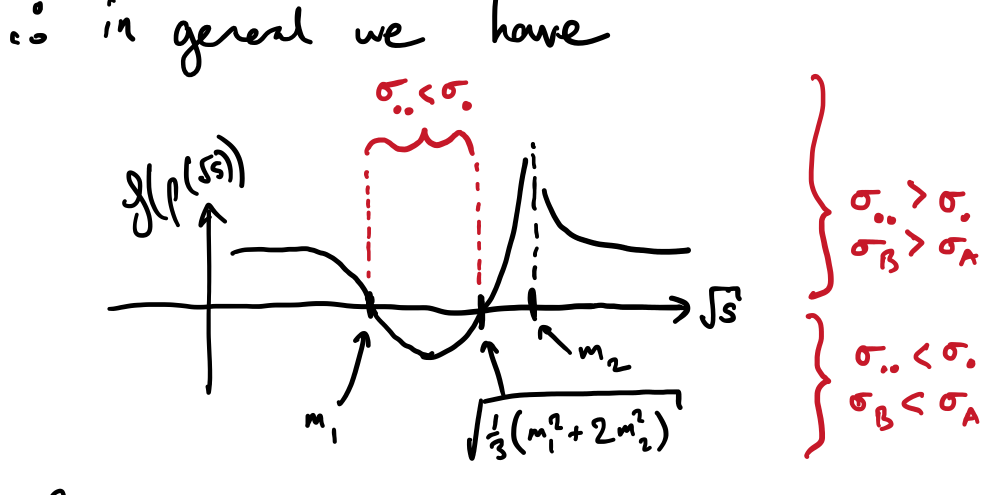
\includegraphics[width=\textwidth]{cropped_working_diag}



\hide{Hence, comparing the two universes:\alig{
|M_{\text{tot(B)}}|^2
- 
|M_{\text{tot(A)}}|^2
&\propto
\left(
e^4|z_{1}|^2
+e^4|z_{2}|^2
+2 e^2 e^2\Re\left[{z_{1}^* z_{2}}\right]
\right)\nonumber
-\left(
e^4|z_{1}|^2
+0^4|z_{2}|^2
+2e^2 0^2 \Re\left[{z_{1}^* z_{2}}\right]
\right)
\\
&\propto
\left(
|z_{1}|^2
+|z_{2}|^2
+2 \Re\left[{z_{1}^*z_{2}}\right]
\right)
-
|z_{1}|^2
\nonumber
\\
&=
|z_{2}|^2
+2 \Re\left[{z_{1}^* z_{2}}\right]
\nonumber
\\
&=
|z_{2}|^2
+2 |z_{1}||z_{2}|\cos\left({\arg {z_2}-\arg{z_1}}\right)
\nonumber
\\
&\propto
\frac {|z_{2}|}{|z_{1}|}
+2 \cos\left({\arg {z_2}-\arg{z_1}}\right)
\nonumber
%\\
%&=
%\frac {|z_{2}|}{|z_{1}|}
%+2 \cos\left({\arg {z_2}-\arg{z_1}}\right)
%\nonumber
\\
&=
\left|\frac {z_{2}}{z_{1}}\right|
+2 \cos\left({\arg \frac{z_2} {z_1}}\right)
\nonumber
\\
&=|\rho| + 2\cos\arg\rho
\\
&\underset{\text{def}}{\equiv} f(\rho)
%&=
%\left| \frac {|1/z_{1}|}{|1|/z_{2}} \right|
%2 \cos\left({\arg {\frac 1 {z_2}}-\arg{\frac 1 {z_1}}}\right)
%\nonumber
%\\
%&=
%\frac {|(s-m_1^2) + i m_1 \Gamma|}{|(s-m_2^2) + i m_2 \Gamma|}
%+2 \cos\left({\arctan {\frac {m_2 \Gamma} {s-m_2^2}}-\arctan{\frac {m_1 \Gamma} %{s-m_1^2}}}\right)
%\nonumber
}where\alig{
\rho &= \frac {z_2}{z_1} = \frac {(s-m_1^2) + i m_1 \Gamma}{(s-m_2^2) + i m_2 \Gamma}.
}
The evaluation of where $f(\rho)$ is posisitive or negative then continues as follows:
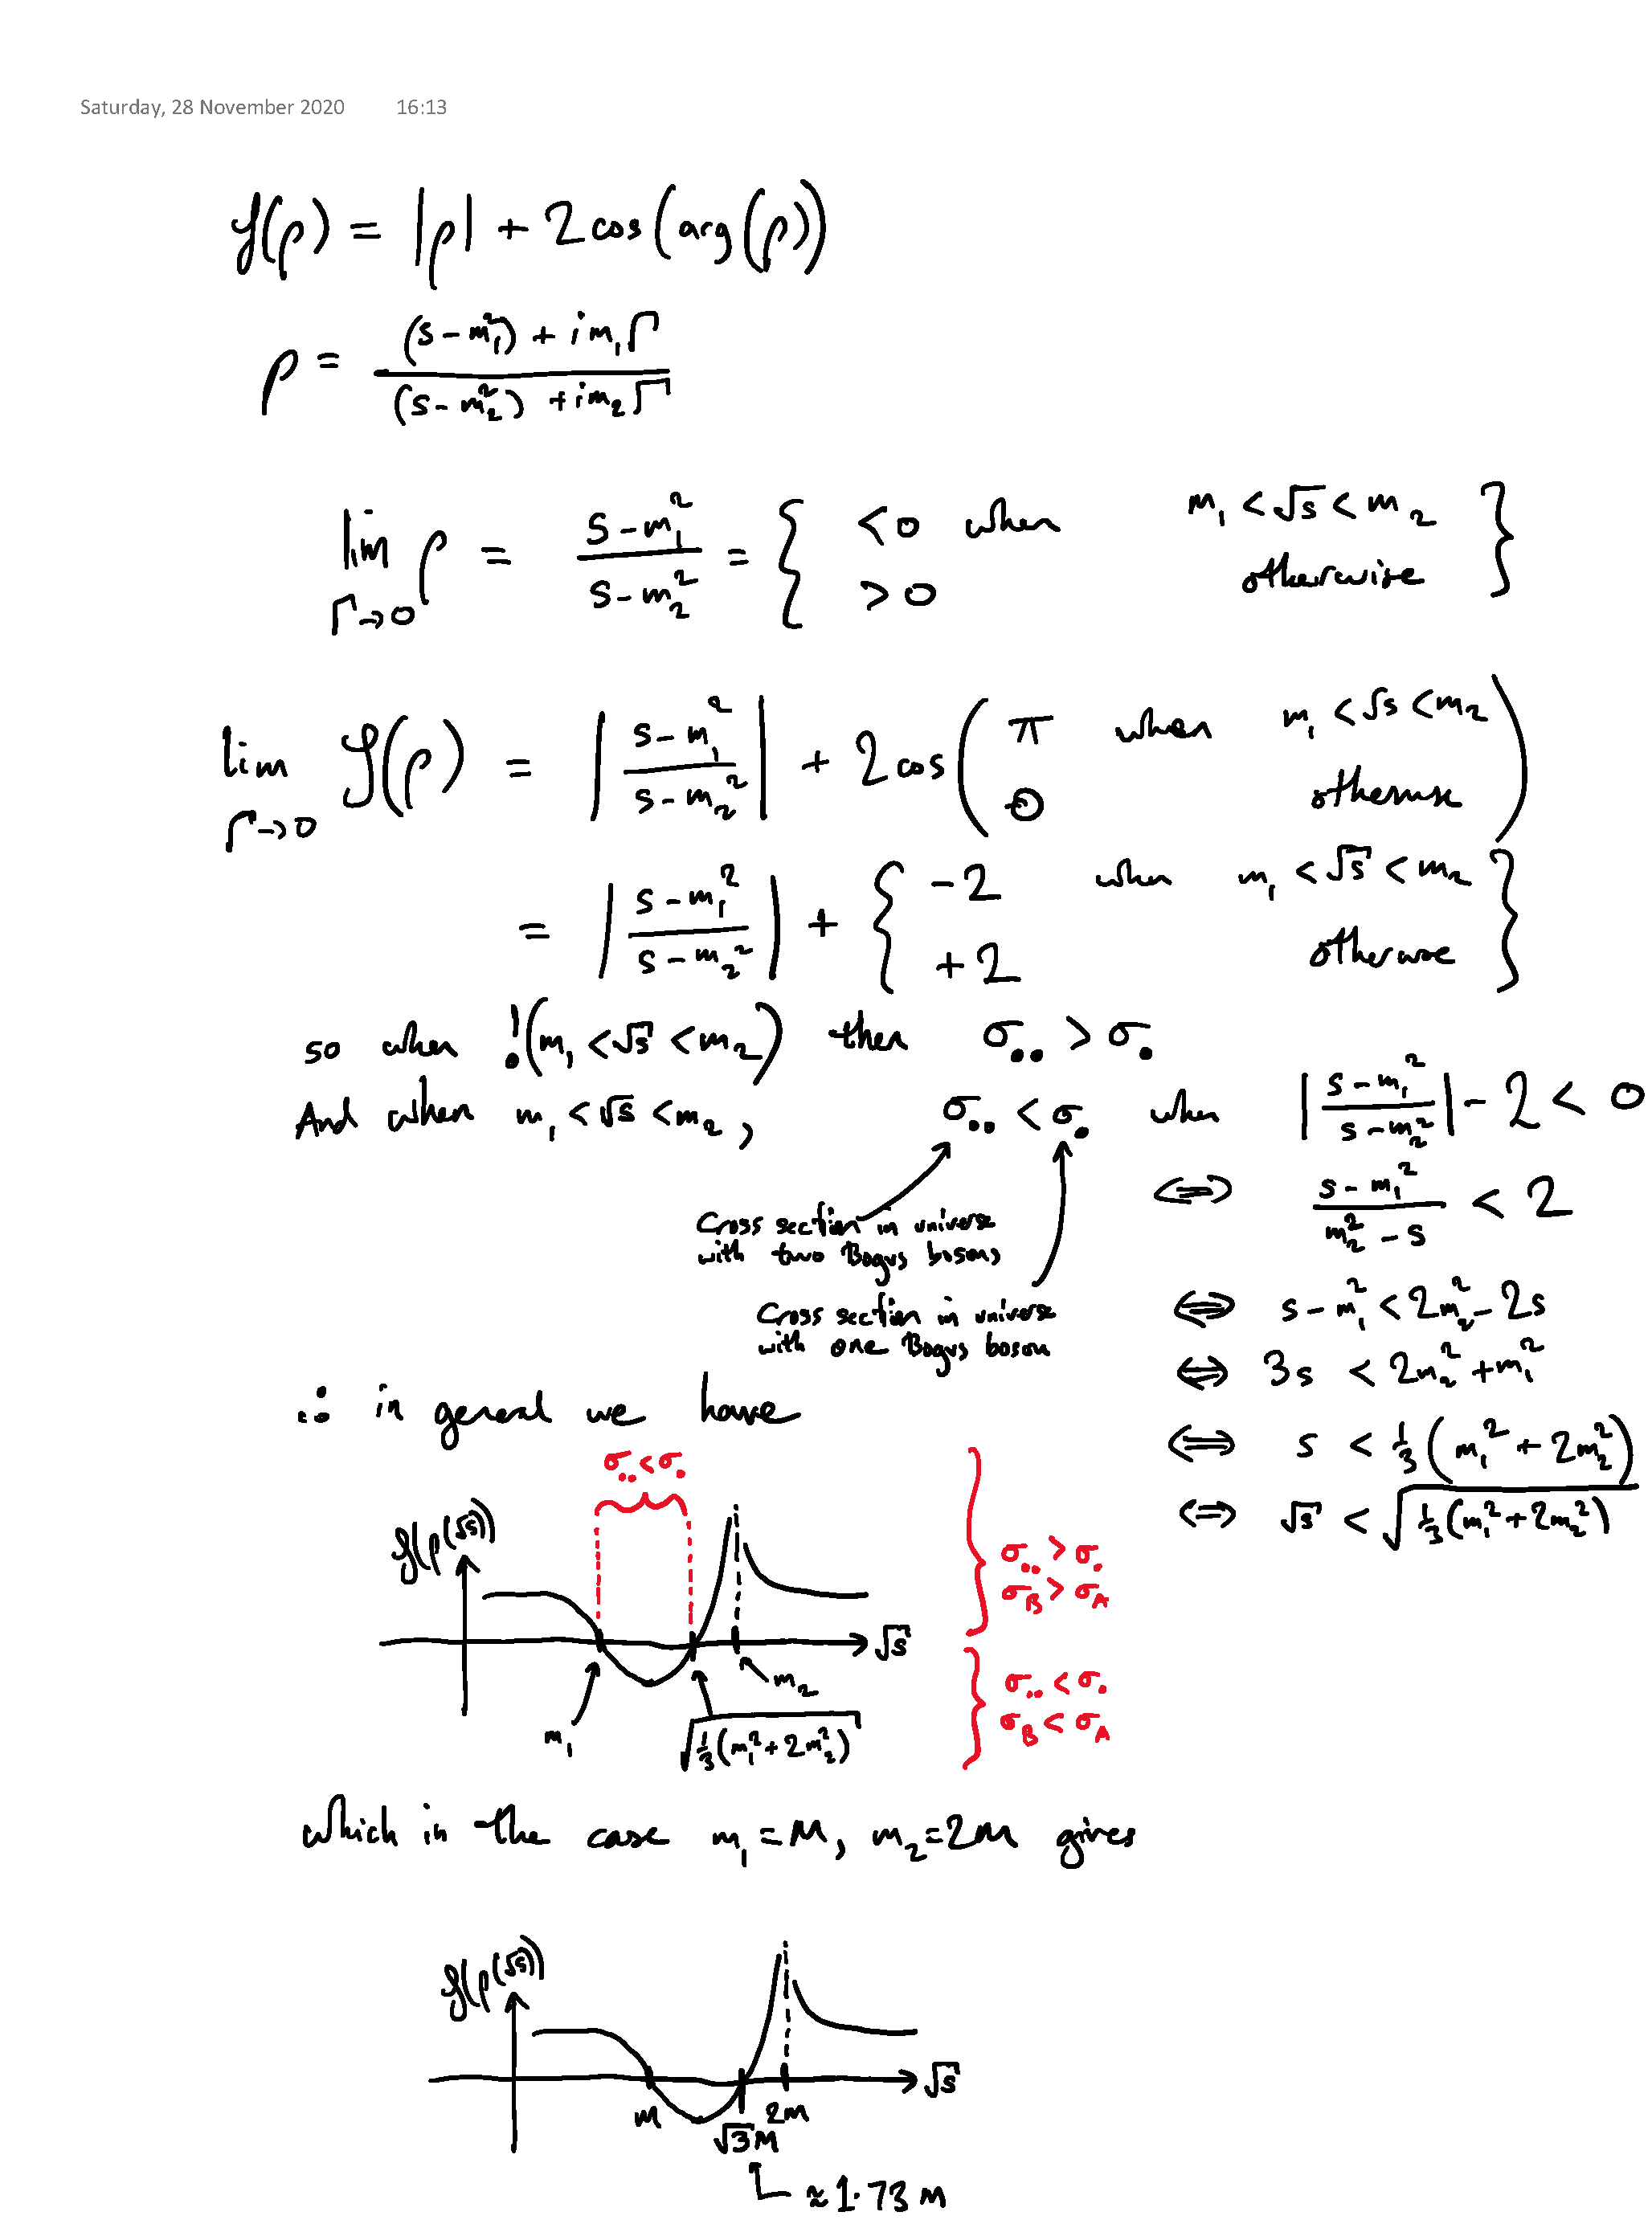
\includegraphics[width=0.9\textwidth]{working}


So the cross section for our process in  universe B is less than in universe A when (and only when) $f(\rho)<0$.  What do we need for this to happen?   Since $|\cos\rho|\le 1$ for all $\rho$, it is clearly an absolute requirement that $\rho$ itself is less than two.  Or put another way:\alig{(|\rho|\ge2) &\implies (f(\rho)\ge0).}   
}
\endanswer
\end{allparts}
A `Bogus $e^+e^-$ Collider' previously only able to reach centre of mass energies of up to $\sqrt s=9m_2$ is upgraded to allow it also to access the region $9m_2<\sqrt s<10 m_2$.  A team of Bogus physicists (who believe themselves to live in Universe B) find that  the $e^+e^-\rightarrow \mu^+\mu^-$ cross section measured by the collider in the new energy region appears    to undershoot the theoretical predictions made by their (previously reliable) Bogus Standard Model.
\begin{allparts}
\part
What conclusion(s) might these physicists draw from the new data? \marks{3}
\answer

In the last part of the question we have seen that between two narrow-width bosons there will inevitably be a region in which interference from the heavier boson makes the total cross section lower than you'd otherwise expect, strange though this seems.  Therefore, the physicists, after first concluding that their standard model was wrong, might tentatively hazard a guess that a new boson was about to appear with a mass somewhere beyond $10m_2$.
\endanswer
\end{allparts}
A %fictional economic meltdown brought about by a fictional government's responses to a fictional plot-device which overly-risk averse external examiners have not permitted me to name on this paper precipitates an imaginary 
funding crisis in physics %which
prohibits the construction of further energy upgrades to the Bogus $e^+e^-$ Collider. 
\begin{allparts}
\part
 What  would you recommend the aforementioned physicists should do to get the most out of the machine they already have? \marks{3}
 \answer
 
 This is a fairly open-ended question, so any sensible thoughtful  answer here will get credit, even if it is not on precisely the same train of thought as the examiner.   Nonetheless, what the examiner has in mind is that candidates will note from the previous answer that there is evidence that there is evidence that there is a new `third' boson just beyond the range of the current collider. Consequently, although they may not be able to make that boson directly, they could perhaps get an indirect measurement of its mass by looking very precisely  deviation of the cross section from their naive two-boson model.  In principle, the shape and size of the deviation completely encapsulates the rest of the spectrum, though in practice the deviations are very small and the extrapolation will have large uncertainties.  In particular, a very heavy boson with a stronger coupling might have similar foothills to a lighter boson with a weaker coupling.  Consequently the uncertainties on the indirect measurements of the coupling and mass of the third boson are likely to be correlated.
 
 It would be interesting to see if any students suggest trying to polarise the beams. [The question notes that \textbf{energy} upgrades are impossible, but doesn't explicitly rule out other forms of upgrade.]
 \endanswer
\end{allparts}
